\section{対象計算領域の設定} \label{sec:domain}
%=======================================================================

\subsection{計算領域と解像度、格子点数、MPIプロセスの関係} \label{subsec:relation_dom_reso}
各設定を行う前に、SCALE-RMでの計算領域、解像度、格子点数、MPIプロセスの関係を整理しておく。
計算領域は、水平格子間隔と格子点数を指定することで決定されるようになっている。
図\ref{fig:domain}は、
計算領域、水平格子間隔、格子数、及びMPIプロセス数の関係を示している。
水平方向に2次元の領域分割を行うことで並列化がなされている。

これらは、\namelist{PARAM_INDEX}内の\nmitem{IMAX}、\nmitem{JMAX}、
\namelist{PARAM_PRC}内の\nmitem{PRC_NUM_X}、\nmitem{PRC_NUM_Y}で
水平格子間隔については、\namelist{PARAM_GRD}内の\nmitem{DX}、\nmitem{DY}で
設定する。

ここで、注意すべきことは、「指定する格子点数は各プロセスが受け持つ値」であることである。
設定する格子数(\nmitem{IMAX}, \nmitem{JMAX}, \nmitem{KMAX})は、
1つのMPIプロセスが担当する格子点数を与える仕様となっている。
すなわち、計算領域は、水平格子間隔、格子点数とともに
各方向のMPIプロセス数を考慮して決定する必要がある。

図\ref{fig:domain}に示すように、
MPIプロセス数が$n$(=\verb|PRC_NUM_X|$\times$\verb|PRC_NUM_Y|)の時、
計算領域は、$x$方向に\verb|PRC_NUM_X|個、$y$方向に\verb|PRC_NUM_Y|個に分割される。
以上の関係から、計算領域全体のそれぞれの方向の格子点数および総格子点数は、
\begin{eqnarray}
&& 領域内x方向の格子数 = \left(\verb|IMAX| \times \verb|PRC_NUM_X|\right)
   \times (\verb|KMAX| )  \label{eq:xgridnum}\\
&& 領域内y方向の格子数 = \left(\verb|JMAX| \times \verb|PRC_NUM_Y|
   \times (\verb|KMAX|\right)  \label{eq:ygridnum}\\
&& 領域内の総格子数 = \left(\verb|IMAX| \times \verb|PRC_NUM_X|\right)
   \times (\verb|JMAX| \times \verb|PRC_NUM_Y|)
   \times (\verb|KMAX| )  \nonumber
\end{eqnarray}
の関係となる。
ここで、\verb|KMAX|は、鉛直方向の格子点数であり、
\namelist{PARAM_INDEX}内の項目で指定されている。
次節以降では、MPIプロセス数、格子数、格子間隔、
それぞれの設定方法について詳しく説明する。

\begin{figure}[h]
\begin{center}
  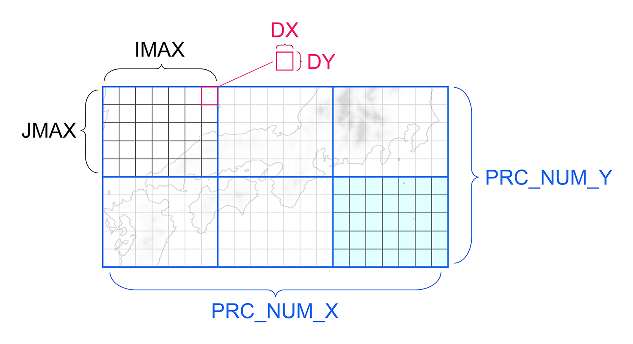
\includegraphics[width=0.8\hsize]{./figure/domain_decomposition.eps}\\
  \caption{計算領域に対する、水平格子間隔(DX, DY)、1MPIプロセスあたりの格子数(IMAX, JMAX)、MPIプロセス数(PRC\_NUM\_X, PRC\_NUM\_Y)の関係。
水色領域は、ある1つのMPIプロセスが担当する領域。}
  \label{fig:domain}
\end{center}
\end{figure}

\subsection{計算領域の設定} \label{subsec:relation_dom_reso2}

\ref{subsec:relation_dom_reso}節で述べた関係が理解できれば、領域の設定は容易である。
すなわち、式(\ref{eq:xgridnum},\ref{eq:ygridnum})を使って、
\begin{eqnarray}
&& x方向の領域の長さ = x方向の格子点数 \times \verb|DX| \nonumber\\
&& y方向の領域の長さ = y方向の格子点数 \times \verb|DY| \nonumber
\end{eqnarray}
となる。ここで、\nmitem{DX,DY}は、後述するように
\namelist{PRAM_GRID}で指定されるものである。
逆算して、解像度と領域の大きさをを決めて、MPIプロセス数が決まると、
ローカルな領域の格子点数が決まる。

\subsection{MPIプロセス数} \label{subsec:relation_dom_reso3}

MPIプロセス数は、設定ファイルの\namelist{PARAM_PRC}で指定する。
先に述べた通り、SCALEの入出力ファイルは、MPIプロセス毎に分割されている。
そのため、MPIプロセス数を変更すると分割ファイル数も必ず変わることになる。
従って、例えば、2-MPI並列用に作成した初期値ファイルは、
4-MPI並列のモデル実行には使用できない。
MPIプロセス数を変更するには、
\verb|pp_***.conf|、\verb|init_***.conf|、\verb|run_***.conf| の
すべてを編集・変更し、\verb|pp|, \verb|init| から行う必要がある。\\

\noindent {\small {\gt
\ovalbox{
\begin{tabularx}{140mm}{lX}
\verb|&PARAM_PRC| & \\
\verb| PRC_NUM_X       = 2,| & ; X方向(東西方向)のMPI並列分割数 \\
\verb| PRC_NUM_Y       = 1,| & ; Y方向(南北方向)のMPI並列分割数 \\
\verb|/|\\
\end{tabularx}
}}}\\


全MPIプロセス数は、\verb|PRC_NUM_X| $\times$ \verb|PRC_NUM_Y|  となり、
上記の例では、$x$方向に2分割、$y$方向に1分割(分割なし)の
2-MPI並列ということになる。

実行時にMPIコマンドに指定するMPIプロセス数は、
この総MPIプロセス数を指定しなければならない。
この条件を満たさない場合は、下記のメッセージが
LOGファイルなどに出力されて計算は行われず、直ちに終了する。

\noindent {\small {\gt
\ovalbox{
\begin{tabularx}{140mm}{l}
\verb|xxx total number of node does not match that requested. Check!| \\
\end{tabularx}
}}}\\





\subsection{水平・鉛直格子数} \label{subsec:relation_dom_reso4}
%-----------------------------------------------------------------------

格子数の設定は、設定ファイル(\verb|***.conf|)の\namelist{PARAM_INDEX}で行う。
\ref{subsec:relation_dom_reso}で詳しく説明したように、以下で設定する水平格子数の値は、
1つのMPIプロセス当たりの値であることに注意が必要である。\\

\noindent {\small {\gt
\ovalbox{
\begin{tabularx}{140mm}{lX}
\verb|&PARAM_INDEX| & \\
\verb| KMAX = 97,|  & 鉛直層数 \\
\verb| IMAX = 20,|  & プロセスあたりのx方向の格子点数 \\
\verb| JMAX = 25,|  & プロセスあたりのy方向の格子点数 \\
\verb|/|\\
\end{tabularx}
}}}\\



\subsection{水平・鉛直格子間隔} \label{sec:gridinterv}
%-----------------------------------------------------------------------
SCALE-RMでは、水平方向には格子点の位置を均等間隔に設定する。
鉛直方向には均等間隔でも任意の格子点位置を直接指定することもできる。
以下で説明する
\textcolor{red}{\bf 格子間隔の設定は、pp\_***.conf、init\_***.conf、run\_***.confの
設定ファイルの間で一致させなければならないことに注意が必要である。}
\ref{subsec:relation_dom_reso}節で述べたように、
以下で設定する値は、MPIプロセス当たりの値であることに注意が必要である。

%-----------------------------------------------------------------------&
第\ref{sec:buffer}節で述べる緩和領域を覗き、
水平格子間隔は等間隔でしか設定できない。
鉛直格子間隔については、任意に定義することが可能である。
すべての方向について等間隔で設定する場合には、以下のように
設定ファイルの\namelist{PARAM_GRID}の\nmitem{DX,DY,DZ}に
それぞれ、東西、南北、鉛直方向の格子間隔を指定する。
単位はmである。

\noindent {\small {\gt
\ovalbox{
\begin{tabularx}{140mm}{lX}
\verb|&PARAM_GRID  | & \\
\verb| DX = 500.D0,| & ; x方向(東西方向)の格子間隔\\
\verb| DY = 500.D0,| & ; y方向(南北方向)の格子間隔\\
\verb| DZ = 500.D0,| & ; z方向(鉛直方向)の格子間隔\\
\verb|/|\\
\end{tabularx}
}}}\\


以下に、鉛直方向での任意の格子点位置を指定する場合の設定を示す。
鉛直方向は、Lorenz格子を採用しており、
速度成分定義格子点とスカラー定義格子点が半格子分ずれた食い違い格子にになっている。
ここでは、スカラー量を定義している格子点をセンターポイントと呼び、
半格子ズレた格子点をフェイスポイントと呼ぶ(図\ref{fig:scale_grid}参照)。

直接格子点の位置を指定する場合は、フェイスポイントの位置を
\namelist{PARAM_GRID}の中の\nmitem{FZ(:)}で配列として与えればよい。
\footnote{指定の際には、シミュレーションの計算精度
(モデルのコンパイル時に指定した浮動小数点の精度。デフォルトでは倍精度)を用いることが望ましい。}
また、\nmitem{FZ(:)}で指定する値の数は、鉛直層数
(\namelist{PARAM_INDEX}の\nmitem{KMAX})と一致させる必要がある。
例として理想実験のチュートリアルのrun.confファイル
(run\_R20kmDX500m.conf)を下記に示す。

\noindent {\small {\gt
\ovalbox{
\begin{tabularx}{140mm}{lX}
\verb|&PARAM_GRID|     & \\
\verb| DX = 500.D0,|   & x方向の格子間隔(等間隔)[m]\\
\verb| DY = 500.D0,|   & y方向の格子間隔(等間隔)[m]\\
\verb| FZ(:) = |       & z方向のフェイスポイントの位置[m] \\
\verb|    80.000000000000000      ,| & \\
\verb|    168.00000190734863      ,| & \\
\verb|    264.80000610351567      ,| & \\
\verb|     〜 中略 〜|           & \\
\verb|    14910.428862936289      ,| & \\
\verb|    15517.262523292475      ,| & \\
\verb|    16215.121232702089      ,| & \\
\verb|    17017.658748523147      ,| & \\
\verb|    17940.576891717363      ,| & \\
\verb|    19001.932756390710      ,| & \\
\verb|    20222.492000765058      ,| & \\
\verb| BUFFER_DZ = 5000.D0,|          & 第\ref{sec:buffer}節参照\\
\verb| BUFFFACT  =   1.0D0,|          & 第\ref{sec:buffer}節参照\\
\verb|/|\\
\end{tabularx}
}}}\\


\begin{figure}[tb]
\begin{center}
  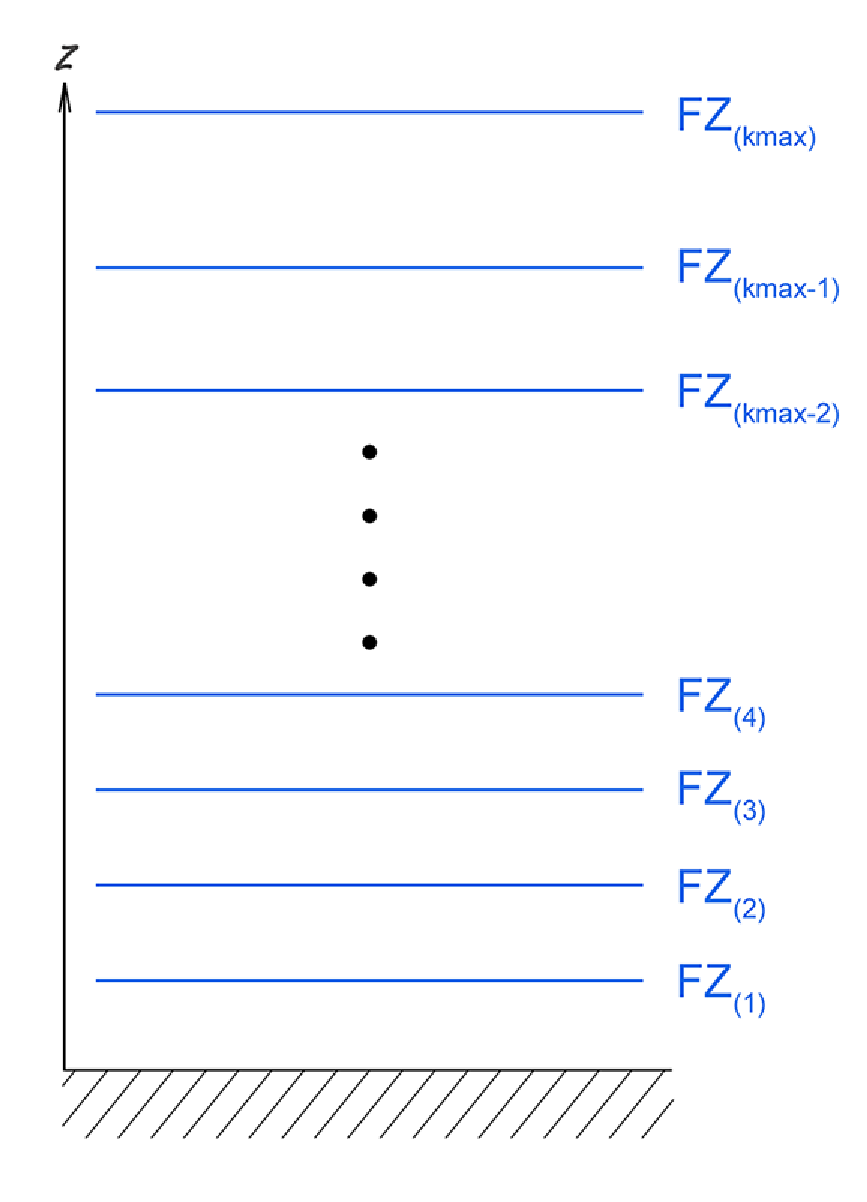
\includegraphics[width=0.4\hsize]{./figure/verticalface.eps}\\
  \caption{SCALE-RMの鉛直格子の定義点。\namelist{PARAM_GRID}で\nmitem{FZ}を指定する時は、ハロを除いた計算領域下端の格子から$k=1$として与える。}
  \label{fig:scale_grid}
\end{center}
\end{figure}
なお、これらの指定では、
標高0mでの格子点として設定され、標高を持つ位置では山岳に沿った座標系によって適切に処理される。


格子点位置は任意に設定できるが、場合によっては計算不安定につながる。
鉛直層の設定については、作成をサポートするツール(\verb|scale/scale-rm/util/makevgrid/|)が
用意されているので参考にされたい。
\footnote{``make\_vgrid.f90''というFortranプログラムと
いくつかのサンプルnamelistが用意されている。}
ツールをコンパイルして実行すれば直ちに設定ファイルに貼り付けて使用できる
\nmitem{FZ(:)}の値が作成される。
